\chapter[相关工作]{相\ 关\ 工\ 作}
\section{引言}
由于目前的分布式存储系统为使用数量非常庞大的存储节点所构成的大规模集群,因此其中的存储介质、服务器和网络等出现故障已经成为常态。根据 Rashmi 等在 Facebook 的数据中心中的研究\cite{rashmi2013solution},其存储系统平均每天会发生 50 起节点不可用事件。因此分布式存储系统的数据备份与恢复是存储系统研究中的重要问题之一。本章首先对存储系统中数据损坏和恢复的方式进行介绍,总结了数据损坏的可能原因以及存储系统的几种数据备份和恢复方式。其次,针对传统数据备份与恢复需要的成本太高或数据冗余度过大等不足之处,介绍了纠删码的编码和解码算法,以及分布式存储系统中基于纠删码的数据备份与恢复算法。最后,针对在基于纠删码的分布式存储系统中数据的修改需要解码并重新编码,造成额外的计算和存储开销的特点,介绍了在基于纠删码的分布式存储系统中文件存储算法的优化。
\section{存储系统中的数据损坏与恢复}
\subsection{存储系统中数据损坏的原因}
在分布式存储系统中,使用了大批量的小型主机取代了集中式存储系统的大型主机,从而减少制造和维护大型主机的成本。然而,小型主机的可靠性和性能一般较大型主机存在一定的差距,也就是说分布式存储系统中节点发生故障的情况是难以避免的,以下是存储系统发生故障的几种常见原因。
\subsubsection{存储介质的物理损坏}
对于软盘、机械硬盘或磁带等存储系统来说,其利用介质的磁性改变存储数据信息。在介质磁性被破坏,或者介质被划伤等等情况发生时,介质中存储数据的单元比如磁道或扇区等,会发生不可逆转的损坏,也就是我们常说的硬盘坏道。部分存储设备会将介质中的坏道进行屏蔽,但是损坏的数据是无法通过正常的数据读取过程读出的。

对于固态硬盘等采用闪存芯片的存储系统来说,其利用浮栅等结构存储电荷,用电荷的存储状态保存数据信息。在介质被多次擦写后,浮栅与沟道之间的氧化层被磨损地越来越严重,最终导致浮栅结构无法可靠地存储电荷,发生数据错误。
\subsubsection{存储设备发生的部件物理故障}
对于硬盘等存储设备来说,除了用于存储数据的磁盘盘片或闪存芯片以外,硬盘内部还会有磁头、电机和电路板等部件,用于从盘片中读写信息,并通过 SATA 或 NVMe 等通信协议与主机通信。若硬盘中的磁头出现偏位或断开,或电路板中的电容发生击穿等,均会导致硬盘出现错误。
\subsubsection{存储设备发生的固件逻辑错误}
对于硬盘等存储设备来说,为了屏蔽坏道以尽可能降低坏道造成的影响,或者对固态硬盘进行磨损平衡以延长使用寿命等目的,硬盘内部一般都会运行着数十万行代码构建的固件\cite{bairavasundaram2008analysis},用以读取存储介质中的数据,并进行映射,然后再将数据传输给主机。如果由于固件 Bug 或者异常断电等原因造成固件逻辑发生错误,则有可能引起数据的丢失。
\subsubsection{文件系统发生的软件错误}
除了存储设备的硬件故障导致数据损毁意外,软件故障也可能导致数据出错或丢失。目前计算机系统中的绝大部分数据均存储于 NTFS、APFS、XFS 或 ext4 等各种类型的文件系统中,由于异常断电、文件系统实现错误等等原因,文件系统也可能出现错误,导致数据发生损坏。
\subsubsection{存储系统使用者的数据误操作}
除了存储系统故障导致的难以预测的数据损坏以外,上层应用或者用户的误操作比如误删除、误格式化或者错误分区等原因,可能导致数据被其使用者自身无意破坏,这也成为了数据丢失的重要原因之一。
\subsection{存储系统中数据恢复的方法}
综上所述,在存储系统中由于存储系统中的硬件故障、软件错误或人为失误等原因,数据损坏是难以避免的,因此在数据损坏前如何进行有效地备份,以及数据发生损坏后如何高效地进行数据恢复,便成为了存储系统研究的重要问题之一。以下我们将分别介绍目前常用的几种数据备份与恢复方法。
\subsubsection{存储设备的物理修复}
针对在数据丢失前未进行有效备份,且数据由于存储设备本身发生故障导致丢失的情况,数据只能通过修复物理设备的方式进行恢复。当硬盘内部的部件发生物理损毁时,或者硬盘内固件发生逻辑错误时,虽然数据能完整地存储于存储介质中,但由于硬盘数据读取所需要的必要部件已经不能正常工作,此时一般只能寻求硬盘生产厂家或专业数据恢复公司的帮助,使用其提供的专用设备,通过开盘直接读取介质内的数据信息,或者通过特殊接口修复固件错误,从而修复损坏设备中的数据。这种方法由于需要较为专业的设备,因此数据恢复的成本较高,而且对于存储介质本身损坏的情形,这种方法不一定能完全有效地恢复数据。
\subsubsection{独立硬盘冗余阵列}
独立硬盘冗余阵列(Redundant Array of Independent Disks,即 RAID)是利用存储虚拟化的思想,将多个物理硬盘组合起来成为虚拟硬盘阵列组,其中除 RAID 0 外,均有不同数量的冗余备份,以保证存储系统中部分存储设备本身发生故障损坏时数据的安全性。RAID 是常用于集中式存储系统中的数据存储方案,操作系统一般将一个 RAID 阵列作为单一的逻辑硬盘操作。
\paragraph{RAID 0}
RAID 0 将两个或以上的存储设备组合起来,共同构成一个大容量的逻辑存储设备。对于 RAID 0 中存储的数据,RAID 控制器将数据分散切分为条块,直接存储于物理磁盘中。这样的结构在数据读写时可以同时在所有硬盘进行并行操作,因此 RAID 0 的读写速度是所有 RAID 级别中最高的。但是 RAID 0 没有存储任何冗余数据,因此不具备检错和纠错的功能。在 RAID 0 的阵列中由于所有数据均分散在所有磁盘上,因此只要其中一个存储设备损坏,整个阵列的所有数据都会丢失,数据安全性极差。
\paragraph{RAID 1}
RAID 1 将两个或以上的硬盘相互作为镜像备份,存储相同的原始数据,当一块硬盘发生损坏,仍可以使用另一块硬盘继续工作。这样的结构在读取数据时也可以同时并发地读取所有硬盘,因此读取性能和 RAID 0 相同,但数据写入时需要同时写入所有硬盘,较单个原始硬盘的写入速度有一定下降。RAID 1 级别的硬盘阵列只要其中一个硬盘正常,便可以正常进行读写,数据安全性最高。但由于 RAID 1 的硬盘之间均互为冗余镜像,因此 RAID 1 的容量为所有单硬盘容量的最小值,硬盘利用率是所有 RAID 级别中最低的。
\paragraph{RAID 2}
RAID 2 使用汉明码(Hamming Code)的方式,将原始数据额外编码,生成一段错误修正码(Error Correction Code,即 ECC),然后通过存储一份原始数据和其错误修正码,实现数据的冗余备份。因此,若要采用 RAID 2,至少需要三个或以上的硬盘设备。RAID 2 在目前的存储系统中较为罕见。
\paragraph{RAID 3}
RAID 3 类似 RAID 2 采用校验码来作为冗余备份数据,但 RAID 3 采用较为简单的异或运算进行校验码的计算,并将数据按比特分割存储于数据盘,校验码单独存放于一块硬盘上。RAID 3 在目前的存储系统中较为罕见。
\paragraph{RAID 4}
RAID 4 采用块交织技术,其采用异或方式生成奇偶校验信息,但在数据分割时按块分割而不是按比特分割,从而保证块的完整性。RAID 4 在目前的存储系统中较为罕见。
\paragraph{RAID 5}
RAID 5 同样采用异或方式生成奇偶校验信息,并作为数据的冗余备份进行存储。其将奇偶校验信息和相对应的数据分别存储于不同的磁盘上,而非单独使用一块硬盘存储校验信息。RAID 5 至少需要三个硬盘,若其中任意一块硬盘发生损坏,均可以利用剩余其他硬盘中的数据和校验信息来恢复重建整个阵列。因此,我们可以认为 RAID 5 是在 RAID 0 的高硬盘利用率和 RAID 1 的高安全性之间权衡的解决方案。
\paragraph{RAID 6}
RAID 6 为了解决 RAID 5 中两块硬盘同时损坏时无法恢复数据的隐患,相比 RAID 5 增加了第二个独立的奇偶校验信息块。两种奇偶校验块通过采用不同的算法\cite{xie2019n,plank2008raid,feng2010eeo,jin2009p},保证任意两块磁盘的同时失效均不会影响数据完整性,大大增加了硬盘阵列的可靠性。由于 RAID 6 增加了额外的奇偶校验,因此需要更大的空间存储校验信息,以及更多的计算资源实现校验码的计算,因此其相对于 RAID 5 来说有更大的 I/O 操作量和计算量,故通常采用专用的硬件 RAID 控制器实现相应计算。
\paragraph{混合 RAID}
通过将不同算法的 RAID 组合使用,可以为存储系统提供更灵活的选择。
\subparagraph{RAID 01}
RAID 01 它将所有的硬盘分为两个 RAID 0 阵列,然后令两个 RAID 0 阵列互为镜像,即 RAID 1。由于这种方式只要有一个硬盘损坏,同组 RAID 0 的其他硬盘也无法正常读写数据,只剩下其他组的硬盘可以工作,因此可靠性较低,在目前的存储系统中较为少用。
\subparagraph{RAID 10}
RAID 10 和 RAID 01 的程序相反,其将所有硬盘分为若干个 RAID 1 阵列,然后将这些 RAID 1 阵列作为 RAID 0 的基本单元进行数据分割存储。这种方式单个硬盘损坏对于其他硬盘没有影响,所有硬盘均可以继续读写数据,阵列可靠性较高。
\subsubsection{文件系统的软件恢复}
针对在数据丢失前未进行有效备份,但数据只是由于文件系统损坏或者使用者误操作引起的逻辑丢失,可以尝试通过数据恢复软件进行数据恢复。对于许多情况下的文件系统损坏和误操作,只是文件系统存储元数据的数据区发生了错误或者被误删除,而真正的用户数据很可能仍然存储于存储设备之上,我们可以通过全盘扫描等方法遍历整个存储设备,尝试越过文件系统的元数据服务,直接读取实际的数据块。这种方法要求数据块本身可以正常读取,也就是说存储设备本身未发生故障,且数据块未被新数据覆盖才能进行数据恢复。
\subsubsection{数据的冗余备份与恢复}
由于存储设备物理修复和文件系统的软件修复均有较为严格的限制条件,且成功率无法保证,因此为了防止数据由于节点故障引起丢失,在分布式存储系统中,一般均会在存储系统的软件层面采用不同类型的冗余备份策略。冗余备份即将部分数据或校验码等冗余存储于多个存储节点,从而保障数据的安全性。
\paragraph{数据的冗余备份机制}
通常的数据冗余备份机制分为两类,即多副本方法和纠删码方法\cite{luo2012summary}。

多副本方法直接将原始数据拷贝多份,每份存储于不同的存储节点的方案,也就是多副本备份方案,便是其中最为简单也最具代表性的。在目前主流分布式存储系统,如 Ceph 分布式文件系统中,一般副本个数均选取为三份,即将三份相同的原始数据分别存储于不同的节点中。显然,三副本方案中冗余备份额外占用的存储空间为原始数据的两倍,即数据冗余度为 $200\%$。这种方法不需要专门的编码和重建算法,因此性能较好,但存储利用率极低。

纠删码方法最早应用于通信传输领域中信息传输过程的检错和纠错问题,后来逐渐扩展到存储系统中,以解决数据存储中的冗余备份问题。纠删码方法相对于多副本方法极大的降低了数据的冗余度,提高了存储资源的利用率。
\paragraph{本地备份与异地备份}
对于冗余备份的数据,若将全部数据均保存于相同的本地机房,假如数据所在机房由于自然灾害或设备损毁整体发生不可用的情况,那么备份数据将同时失效。因此在重要的存储系统中,一般均会采用异地备份进行容灾。异地备份可以选择多副本方法或纠删码方法构造冗余数据,然后将冗余数据存储于不同机房甚至不同城市的其他存储集群中,来保障数据的安全。
\paragraph{在线备份与离线备份}
对于重要的数据来说,除了需要避免存储系统本身的故障导致的数据丢失以外,还需要保证在系统被攻击、应用程序出错或者使用者误操作等情况发生时的数据安全性。由于在线备份的数据无法保障上述情况发生时的数据安全,因此常用离线备份的策略,将存储系统中某个时间点的数据全部拷贝出来,生成一份数据镜像存储到外部的存储设备中,并将该备份存储设备脱机保存,以保证即使所有在线备份的数据都被破坏时,也可以从离线备份中进行数据恢复。由于在线备份无法实时进行,因此使用离线备份可能会导致部分最新产生的数据丢失,故从离线备份的副本中恢复一般被认为是存储系统数据安全的最后一道防线,仅在其他方法均无法有效地恢复数据时才会采用。
\section{存储系统中的纠删码编码技术}
\subsection{阵列码}
阵列码(Array Codes)是一种基于异或(XOR)运算的纠删码编码方式,分为横式阵列码和纵式阵列码两种。这类编码由于计算简便\cite{yuan2019research},被广泛应用于 RAID 6 中\cite{xie2019n,plank2008raid,feng2010eeo,jin2009p}。
\subsubsection{横式阵列码}
横式阵列码(Horizontal Parity Array Codes)是指冗余编码块和数据编码块相互独立,分别单独进行存储的阵列码编码方式。由于其冗余编码的存储是独立的,因而具有良好的可扩展性。典型的横式阵列码的容错率都不是很大,其中容错率为 2 的编码包括 EVENODD 编码\cite{blaum1995evenodd}和 RDP 编码\cite{corbett2004row}等,容错率大于 2 的编码较少,主要包括 STAR 编码\cite{huang2008star}等。

图 \ref{p10} 和图 \ref{p11} 分别给出了典型的两种横式阵列码 EVENODD 编码和 RDP 编码的示意图\cite{xiang2011hybrid},其中 EVENODD 编码是最早出现的阵列码编码方式。这些编码体系均要求数据块的个数必须与硬盘数量相匹配,且不能实现对任意数量硬盘的编码。在存储空间的利用率方面,由于这些编码的存储效率均达到了理论上的最优,因此均为 MDS 编码(Maximum Distance Separable Codes)。

\begin{figure}[!htb]
\centering
\resizebox{.8\textwidth}{!}{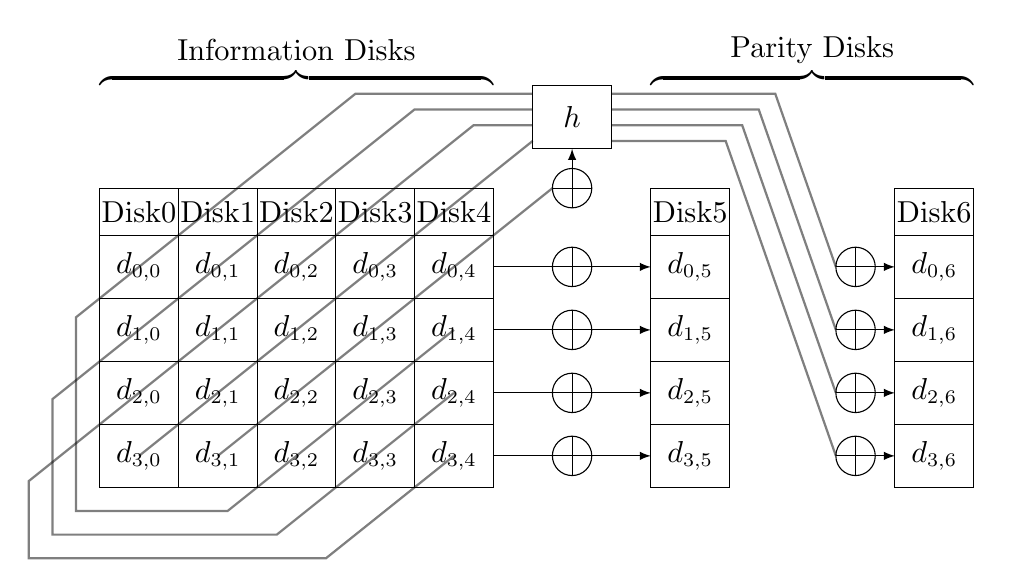
\begin{tikzpicture}
\fill [color=white,opacity=0] (0, 0) rectangle (12, 6.7);

\draw (0.9, 0.9) rectangle (5.9, 4.7);
\draw (0.9, 1.7) -- (5.9, 1.7);
\draw (0.9, 2.5) -- (5.9, 2.5);
\draw (0.9, 3.3) -- (5.9, 3.3);
\draw (0.9, 4.1) -- (5.9, 4.1);
\draw (1.9, 0.9) -- (1.9, 4.7);
\draw (2.9, 0.9) -- (2.9, 4.7);
\draw (3.9, 0.9) -- (3.9, 4.7);
\draw (4.9, 0.9) -- (4.9, 4.7);
\node at (1.4, 4.4) [font=\fontsize{10.5pt}{20pt}\selectfont] {Disk0};
\node at (2.4, 4.4) [font=\fontsize{10.5pt}{20pt}\selectfont] {Disk1};
\node at (3.4, 4.4) [font=\fontsize{10.5pt}{20pt}\selectfont] {Disk2};
\node at (4.4, 4.4) [font=\fontsize{10.5pt}{20pt}\selectfont] {Disk3};
\node at (5.4, 4.4) [font=\fontsize{10.5pt}{20pt}\selectfont] {Disk4};
\node at (1.4, 3.7) [font=\fontsize{10.5pt}{20pt}\selectfont] {$d_{0,0}$};
\node at (2.4, 3.7) [font=\fontsize{10.5pt}{20pt}\selectfont] {$d_{0,1}$};
\node at (3.4, 3.7) [font=\fontsize{10.5pt}{20pt}\selectfont] {$d_{0,2}$};
\node at (4.4, 3.7) [font=\fontsize{10.5pt}{20pt}\selectfont] {$d_{0,3}$};
\node at (5.4, 3.7) [font=\fontsize{10.5pt}{20pt}\selectfont] {$d_{0,4}$};
\node at (1.4, 2.9) [font=\fontsize{10.5pt}{20pt}\selectfont] {$d_{1,0}$};
\node at (2.4, 2.9) [font=\fontsize{10.5pt}{20pt}\selectfont] {$d_{1,1}$};
\node at (3.4, 2.9) [font=\fontsize{10.5pt}{20pt}\selectfont] {$d_{1,2}$};
\node at (4.4, 2.9) [font=\fontsize{10.5pt}{20pt}\selectfont] {$d_{1,3}$};
\node at (5.4, 2.9) [font=\fontsize{10.5pt}{20pt}\selectfont] {$d_{1,4}$};
\node at (1.4, 2.1) [font=\fontsize{10.5pt}{20pt}\selectfont] {$d_{2,0}$};
\node at (2.4, 2.1) [font=\fontsize{10.5pt}{20pt}\selectfont] {$d_{2,1}$};
\node at (3.4, 2.1) [font=\fontsize{10.5pt}{20pt}\selectfont] {$d_{2,2}$};
\node at (4.4, 2.1) [font=\fontsize{10.5pt}{20pt}\selectfont] {$d_{2,3}$};
\node at (5.4, 2.1) [font=\fontsize{10.5pt}{20pt}\selectfont] {$d_{2,4}$};
\node at (1.4, 1.3) [font=\fontsize{10.5pt}{20pt}\selectfont] {$d_{3,0}$};
\node at (2.4, 1.3) [font=\fontsize{10.5pt}{20pt}\selectfont] {$d_{3,1}$};
\node at (3.4, 1.3) [font=\fontsize{10.5pt}{20pt}\selectfont] {$d_{3,2}$};
\node at (4.4, 1.3) [font=\fontsize{10.5pt}{20pt}\selectfont] {$d_{3,3}$};
\node at (5.4, 1.3) [font=\fontsize{10.5pt}{20pt}\selectfont] {$d_{3,4}$};
\draw (7.9, 0.9) rectangle (8.9, 4.7);
\draw (7.9, 1.7) -- (8.9, 1.7);
\draw (7.9, 2.5) -- (8.9, 2.5);
\draw (7.9, 3.3) -- (8.9, 3.3);
\draw (7.9, 4.1) -- (8.9, 4.1);
\node at (8.4, 4.4) [font=\fontsize{10.5pt}{20pt}\selectfont] {Disk5};
\node at (8.4, 3.7) [font=\fontsize{10.5pt}{20pt}\selectfont] {$d_{0,5}$};
\node at (8.4, 2.9) [font=\fontsize{10.5pt}{20pt}\selectfont] {$d_{1,5}$};
\node at (8.4, 2.1) [font=\fontsize{10.5pt}{20pt}\selectfont] {$d_{2,5}$};
\node at (8.4, 1.3) [font=\fontsize{10.5pt}{20pt}\selectfont] {$d_{3,5}$};
\draw (11, 0.9) rectangle (12, 4.7);
\draw (11, 1.7) -- (12, 1.7);
\draw (11, 2.5) -- (12, 2.5);
\draw (11, 3.3) -- (12, 3.3);
\draw (11, 4.1) -- (12, 4.1);
\node at (11.5, 4.4) [font=\fontsize{10.5pt}{20pt}\selectfont] {Disk6};
\node at (11.5, 3.7) [font=\fontsize{10.5pt}{20pt}\selectfont] {$d_{0,6}$};
\node at (11.5, 2.9) [font=\fontsize{10.5pt}{20pt}\selectfont] {$d_{1,6}$};
\node at (11.5, 2.1) [font=\fontsize{10.5pt}{20pt}\selectfont] {$d_{2,6}$};
\node at (11.5, 1.3) [font=\fontsize{10.5pt}{20pt}\selectfont] {$d_{3,6}$};
\draw (6.4, 5.2) rectangle (7.4, 6);
\node at (6.9, 5.6) [font=\fontsize{10.5pt}{20pt}\selectfont] {$h$};
\draw [thick,opacity=0.5] (5.4, 1.3) -- (3.775, 0) -- (0, 0) -- (0, 0.98) -- (5.65, 5.5) -- (6.4, 5.5);
\draw [thick,opacity=0.5] (5.4, 2.1) -- (3.15, 0.3) -- (0.3, 0.3) -- (0.3, 2.02) -- (4.9, 5.7) -- (6.4, 5.7);
\draw [thick,opacity=0.5] (5.4, 2.9) -- (2.525, 0.6) -- (0.6, 0.6) -- (0.6, 3.06) -- (4.15, 5.9) -- (6.4, 5.9);
\draw [thick,opacity=0.5] (2.4, 1.3) -- (6.65, 4.7);
\draw [thick,opacity=0.5] (1.4, 1.3) -- (6.4, 5.3);
\draw (6.9, 4.7) circle (0.25);
\draw (6.9, 3.7) circle (0.25);
\draw (6.9, 2.9) circle (0.25);
\draw (6.9, 2.1) circle (0.25);
\draw (6.9, 1.3) circle (0.25);
\draw (6.65, 4.7) -- (7.15, 4.7);
\draw [-latex] (6.9, 4.45) -- (6.9, 5.2);
\draw [-latex] (5.9, 3.7) -- (7.9, 3.7);
\draw (6.9, 3.45) -- (6.9, 3.95);
\draw [-latex] (5.9, 2.9) -- (7.9, 2.9);
\draw (6.9, 2.65) -- (6.9, 3.15);
\draw [-latex] (5.9, 2.1) -- (7.9, 2.1);
\draw (6.9, 1.85) -- (6.9, 2.35);
\draw [-latex] (5.9, 1.3) -- (7.9, 1.3);
\draw (6.9, 1.05) -- (6.9, 1.55);
\draw (10.5, 3.7) circle (0.25);
\draw (10.5, 2.9) circle (0.25);
\draw (10.5, 2.1) circle (0.25);
\draw (10.5, 1.3) circle (0.25);
\draw [thick,opacity=0.5] (7.4, 5.9) -- (9.48, 5.9) -- (10.25, 3.7);
\draw [thick,opacity=0.5] (7.4, 5.7) -- (9.27, 5.7) -- (10.25, 2.9);
\draw [thick,opacity=0.5] (7.4, 5.5) -- (9.06, 5.5) -- (10.25, 2.1);
\draw [thick,opacity=0.5] (7.4, 5.3) -- (8.85, 5.3) -- (10.25, 1.3);
\draw [-latex] (10.25, 3.7) -- (11, 3.7);
\draw (10.5, 3.45) -- (10.5, 3.95);
\draw [-latex] (10.25, 2.9) -- (11, 2.9);
\draw (10.5, 2.65) -- (10.5, 3.15);
\draw [-latex] (10.25, 2.1) -- (11, 2.1);
\draw (10.5, 1.85) -- (10.5, 2.35);
\draw [-latex] (10.25, 1.3) -- (11, 1.3);
\draw (10.5, 1.05) -- (10.5, 1.55);
\node at (3.4, 6.1) [rotate=180] {$\underbrace{\hspace{5cm}}$};
\node at (3.4, 6.45) [font=\fontsize{10.5pt}{20pt}\selectfont] {Information Disks};
\node at (9.95, 6.1) [rotate=180] {$\underbrace{\hspace{4.1cm}}$};
\node at (9.95, 6.45) [font=\fontsize{10.5pt}{20pt}\selectfont] {Parity Disks};
\end{tikzpicture}
}
\caption{EVENODD 编码示意}
\label{p10}
\end{figure}

\begin{figure}[!htb]
\centering
\resizebox{.8\textwidth}{!}{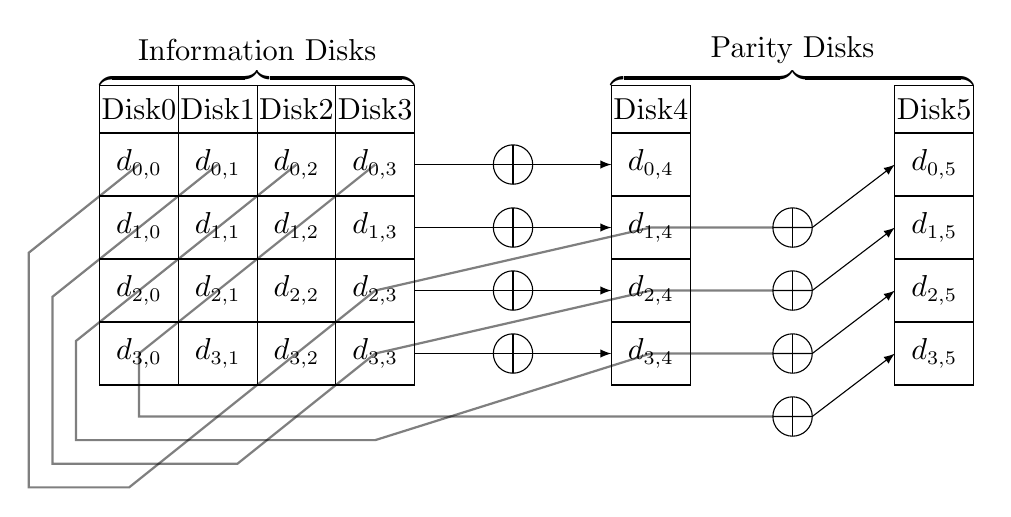
\begin{tikzpicture}
\fill [color=white,opacity=0] (0, 0) rectangle (12, 5.8);

\draw (0.9, 1.3) rectangle (4.9, 5.1);
\draw (0.9, 2.1) -- (4.9, 2.1);
\draw (0.9, 2.9) -- (4.9, 2.9);
\draw (0.9, 3.7) -- (4.9, 3.7);
\draw (0.9, 4.5) -- (4.9, 4.5);
\draw (1.9, 1.3) -- (1.9, 5.1);
\draw (2.9, 1.3) -- (2.9, 5.1);
\draw (3.9, 1.3) -- (3.9, 5.1);
\node at (1.4, 4.8) [font=\fontsize{10.5pt}{20pt}\selectfont] {Disk0};
\node at (2.4, 4.8) [font=\fontsize{10.5pt}{20pt}\selectfont] {Disk1};
\node at (3.4, 4.8) [font=\fontsize{10.5pt}{20pt}\selectfont] {Disk2};
\node at (4.4, 4.8) [font=\fontsize{10.5pt}{20pt}\selectfont] {Disk3};
\node at (1.4, 4.1) [font=\fontsize{10.5pt}{20pt}\selectfont] {$d_{0,0}$};
\node at (2.4, 4.1) [font=\fontsize{10.5pt}{20pt}\selectfont] {$d_{0,1}$};
\node at (3.4, 4.1) [font=\fontsize{10.5pt}{20pt}\selectfont] {$d_{0,2}$};
\node at (4.4, 4.1) [font=\fontsize{10.5pt}{20pt}\selectfont] {$d_{0,3}$};
\node at (1.4, 3.3) [font=\fontsize{10.5pt}{20pt}\selectfont] {$d_{1,0}$};
\node at (2.4, 3.3) [font=\fontsize{10.5pt}{20pt}\selectfont] {$d_{1,1}$};
\node at (3.4, 3.3) [font=\fontsize{10.5pt}{20pt}\selectfont] {$d_{1,2}$};
\node at (4.4, 3.3) [font=\fontsize{10.5pt}{20pt}\selectfont] {$d_{1,3}$};
\node at (1.4, 2.5) [font=\fontsize{10.5pt}{20pt}\selectfont] {$d_{2,0}$};
\node at (2.4, 2.5) [font=\fontsize{10.5pt}{20pt}\selectfont] {$d_{2,1}$};
\node at (3.4, 2.5) [font=\fontsize{10.5pt}{20pt}\selectfont] {$d_{2,2}$};
\node at (4.4, 2.5) [font=\fontsize{10.5pt}{20pt}\selectfont] {$d_{2,3}$};
\node at (1.4, 1.7) [font=\fontsize{10.5pt}{20pt}\selectfont] {$d_{3,0}$};
\node at (2.4, 1.7) [font=\fontsize{10.5pt}{20pt}\selectfont] {$d_{3,1}$};
\node at (3.4, 1.7) [font=\fontsize{10.5pt}{20pt}\selectfont] {$d_{3,2}$};
\node at (4.4, 1.7) [font=\fontsize{10.5pt}{20pt}\selectfont] {$d_{3,3}$};
\draw (7.4, 1.3) rectangle (8.4, 5.1);
\draw (7.4, 2.1) -- (8.4, 2.1);
\draw (7.4, 2.9) -- (8.4, 2.9);
\draw (7.4, 3.7) -- (8.4, 3.7);
\draw (7.4, 4.5) -- (8.4, 4.5);
\node at (7.9, 4.8) [font=\fontsize{10.5pt}{20pt}\selectfont] {Disk4};
\node at (7.9, 4.1) [font=\fontsize{10.5pt}{20pt}\selectfont] {$d_{0,4}$};
\node at (7.9, 3.3) [font=\fontsize{10.5pt}{20pt}\selectfont] {$d_{1,4}$};
\node at (7.9, 2.5) [font=\fontsize{10.5pt}{20pt}\selectfont] {$d_{2,4}$};
\node at (7.9, 1.7) [font=\fontsize{10.5pt}{20pt}\selectfont] {$d_{3,4}$};
\draw (11, 1.3) rectangle (12, 5.1);
\draw (11, 2.1) -- (12, 2.1);
\draw (11, 2.9) -- (12, 2.9);
\draw (11, 3.7) -- (12, 3.7);
\draw (11, 4.5) -- (12, 4.5);
\node at (11.5, 4.8) [font=\fontsize{10.5pt}{20pt}\selectfont] {Disk5};
\node at (11.5, 4.1) [font=\fontsize{10.5pt}{20pt}\selectfont] {$d_{0,5}$};
\node at (11.5, 3.3) [font=\fontsize{10.5pt}{20pt}\selectfont] {$d_{1,5}$};
\node at (11.5, 2.5) [font=\fontsize{10.5pt}{20pt}\selectfont] {$d_{2,5}$};
\node at (11.5, 1.7) [font=\fontsize{10.5pt}{20pt}\selectfont] {$d_{3,5}$};
\draw (6.15, 4.1) circle (0.25);
\draw (6.15, 3.3) circle (0.25);
\draw (6.15, 2.5) circle (0.25);
\draw (6.15, 1.7) circle (0.25);
\draw (6.15, 3.85) -- (6.15, 4.35);
\draw [-latex] (4.9, 4.1) -- (7.4, 4.1);
\draw (6.15, 3.05) -- (6.15, 3.55);
\draw [-latex] (4.9, 3.3) -- (7.4, 3.3);
\draw (6.15, 2.25) -- (6.15, 2.75);
\draw [-latex] (4.9, 2.5) -- (7.4, 2.5);
\draw (6.15, 1.45) -- (6.15, 1.95);
\draw [-latex] (4.9, 1.7) -- (7.4, 1.7);
\draw (9.7, 3.3) circle (0.25);
\draw (9.7, 2.5) circle (0.25);
\draw (9.7, 1.7) circle (0.25);
\draw (9.7, 0.9) circle (0.25);
\draw (9.7, 3.05) -- (9.7, 3.55);
\draw [-latex] (9.45, 3.3) -- (9.95, 3.3) -- (11, 4.1);
\draw (9.7, 2.25) -- (9.7, 2.75);
\draw [-latex] (9.45, 2.5) -- (9.95, 2.5) -- (11, 3.3);
\draw (9.7, 1.45) -- (9.7, 1.95);
\draw [-latex] (9.45, 1.7) -- (9.95, 1.7) -- (11, 2.5);
\draw (9.7, 0.65) -- (9.7, 1.15);
\draw [-latex] (9.45, 0.9) -- (9.95, 0.9) -- (11, 1.7);
\draw [thick,opacity=0.5] (1.4, 4.1) -- (0, 2.98) -- (0, 0) -- (1.275, 0) -- (4.4, 2.5) -- (7.9, 3.3) -- (9.45, 3.3);
\draw [thick,opacity=0.5] (2.4, 4.1) -- (0.3, 2.42) -- (0.3, 0.3) -- (2.65, 0.3) -- (4.4, 1.7) -- (7.9, 2.5) -- (9.45, 2.5);
\draw [thick,opacity=0.5] (3.4, 4.1) -- (0.6, 1.86) -- (0.6, 0.6) -- (4.4, 0.6) -- (7.9, 1.7) -- (9.45, 1.7);
\draw [thick,opacity=0.5] (4.4, 4.1) -- (1.4, 1.7) -- (1.4, 0.9) -- (9.45, 0.9);
\node at (2.9, 5.2) [rotate=180] {$\underbrace{\hspace{4cm}}$};
\node at (2.9, 5.55) [font=\fontsize{10.5pt}{20pt}\selectfont] {Information Disks};
\node at (9.7, 5.2) [rotate=180] {$\underbrace{\hspace{4.6cm}}$};
\node at (9.7, 5.55) [font=\fontsize{10.5pt}{20pt}\selectfont] {Parity Disks};
\end{tikzpicture}
}
\caption{RDP 编码示意}
\label{p11}
\end{figure}
\subsubsection{纵式阵列码}
纵式阵列码(Vertical Parity Array Codes)与横式阵列码不同,其并不将冗余编码块与数据编码块单独存储于不同的硬盘上,而是直接将冗余数据存储于原始数据块的内部。在纵式阵列码的数据块中,既存储了原始数据,又存储了冗余编码。由于冗余数据分散存储与各个硬盘,因此不存在横式阵列码中冗余数据盘在数据写入时的瓶颈问题。但纵式阵列码中的硬盘之间依赖性强,可扩展性较差。目前的纵式阵列码主要包括 X-code 编码\cite{xu1999x}和 WEAVER 编码\cite{hafner2005weaver}等。

图 \ref{p12} 给出了 X-code 编码示意图\cite{shen2015hv}。在由 $n$ 块磁盘组成的 X-code 的编码中,每块磁盘中包含 $n-2$ 个数据块和 $2$ 个冗余编码块,其中要求 $n$ 必须是一个大于 2 的素数。X-code 编码具有理论上最优的运算效率,且在存储利用率上 X-code 也是 MDS 的编码,但由于其中 $n$ 必须为素数的限制导致其可扩展性很差。

\begin{figure}[!htb]
\centering
\resizebox{.8\textwidth}{!}{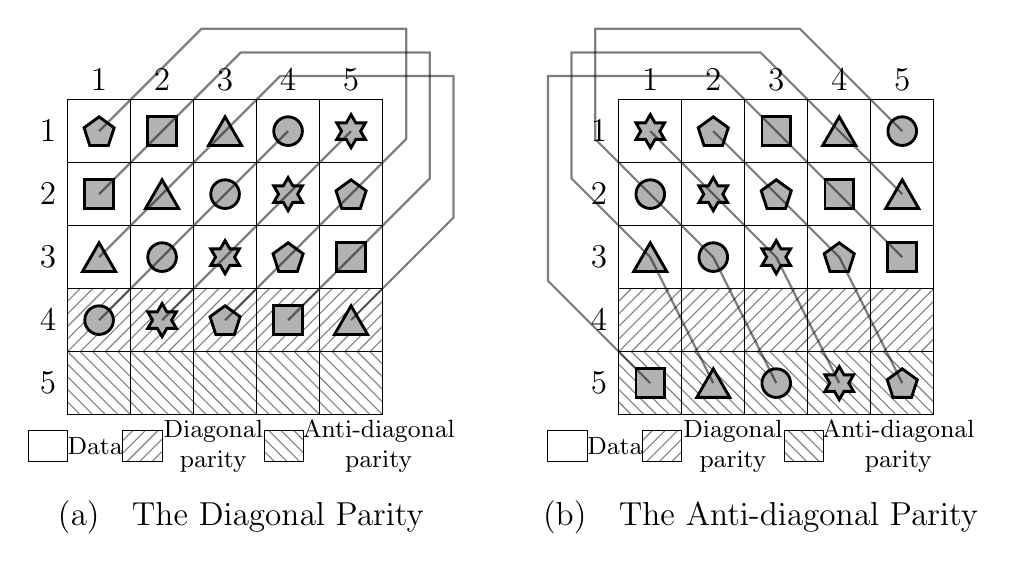
\begin{tikzpicture}
\fill [color=white,opacity=0] (0, 0) rectangle (12, 6.7);
\newcommand\shapeA{\resizebox{!}{0.4cm}{\tikz\filldraw [fill=black!30!white, line width=0.1809cm] (0, 1) -- (-0.951, 0.309) -- (-0.588, -0.809) -- (0.588, -0.809) -- (0.951, 0.309) -- cycle;}}
\newcommand\shapeB{\resizebox{!}{0.4cm}{\tikz\filldraw [fill=black!30!white, line width=0.1414cm] (0.707, 0.707) -- (-0.707, 0.707) -- (-0.707, -0.707) -- (0.707, -0.707) -- cycle;}}
\newcommand\shapeC{\resizebox{!}{0.4cm}{\tikz\filldraw [fill=black!30!white, line width=0.15cm] (0, 1) -- (0.866, -0.5) -- (-0.866, -0.5) -- cycle;}}
\newcommand\shapeD{\resizebox{!}{0.4cm}{\tikz\filldraw [fill=black!30!white, line width=0.2cm] (0, 0) circle (1);}}
\newcommand\shapeE{\resizebox{0.4cm}{!}{\tikz\filldraw [fill=black!30!white, line width=0.1732cm] (0, 1) -- (0.289, 0.5) -- (0.866, 0.5) -- (0.577, 0) -- (0.866, -0.5) -- (0.289, -0.5) -- (0, -1) -- (-0.289, -0.5) -- (-0.866, -0.5) -- (-0.577, 0) -- (-0.866, 0.5) -- (-0.289, 0.5) -- cycle;}}

\node at (2.7, 0.5) [font=\fontsize{12pt}{20pt}\selectfont] {(a){\quad}The Diagonal Parity};
\node at (9.3, 0.5) [font=\fontsize{12pt}{20pt}\selectfont] {(b){\quad}The Anti-diagonal Parity};

\foreach \x in {0,...,20} {
\draw [color=black!50!white] (1.3+0.16*\x, 3.4) -- (0.5+0.16*\x, 2.6);
\draw [color=black!50!white] (8.3+0.16*\x, 3.4) -- (7.5+0.16*\x, 2.6);
\draw [color=black!50!white] (1.3+0.16*\x, 1.8) -- (0.5+0.16*\x, 2.6);
\draw [color=black!50!white] (8.3+0.16*\x, 1.8) -- (7.5+0.16*\x, 2.6);
}
\foreach \x in {1,...,4} {
\draw [color=black!50!white] (1.3-0.16*\x, 3.4) -- (0.5, 2.6+0.16*\x);
\draw [color=black!50!white] (4.5-0.16*\x, 2.6) -- (4.5, 2.6+0.16*\x);
\draw [color=black!50!white] (8.3-0.16*\x, 3.4) -- (7.5, 2.6+0.16*\x);
\draw [color=black!50!white] (11.5-0.16*\x, 2.6) -- (11.5, 2.6+0.16*\x);
\draw [color=black!50!white] (1.3-0.16*\x, 1.8) -- (0.5, 2.6-0.16*\x);
\draw [color=black!50!white] (4.5-0.16*\x, 2.6) -- (4.5, 2.6-0.16*\x);
\draw [color=black!50!white] (8.3-0.16*\x, 1.8) -- (7.5, 2.6-0.16*\x);
\draw [color=black!50!white] (11.5-0.16*\x, 2.6) -- (11.5, 2.6-0.16*\x);
}

\draw [color=black!50!white] (1.33, 1.6) -- (1.2, 1.47);
\draw [color=black!50!white] (1.49, 1.6) -- (1.2, 1.31);
\draw [color=black!50!white] (1.65, 1.6) -- (1.25, 1.2);
\draw [color=black!50!white] (1.7, 1.49) -- (1.41, 1.2);
\draw [color=black!50!white] (1.7, 1.33) -- (1.57, 1.2);

\draw [color=black!50!white] (3.13, 1.2) -- (3, 1.33);
\draw [color=black!50!white] (3.29, 1.2) -- (3, 1.49);
\draw [color=black!50!white] (3.45, 1.2) -- (3.05, 1.6);
\draw [color=black!50!white] (3.5, 1.31) -- (3.21, 1.6);
\draw [color=black!50!white] (3.5, 1.47) -- (3.37, 1.6);

\draw [color=black!50!white] (7.93, 1.6) -- (7.8, 1.47);
\draw [color=black!50!white] (8.09, 1.6) -- (7.8, 1.31);
\draw [color=black!50!white] (8.25, 1.6) -- (7.85, 1.2);
\draw [color=black!50!white] (8.3, 1.49) -- (8.01, 1.2);
\draw [color=black!50!white] (8.3, 1.33) -- (8.17, 1.2);

\draw [color=black!50!white] (9.73, 1.2) -- (9.6, 1.33);
\draw [color=black!50!white] (9.89, 1.2) -- (9.6, 1.49);
\draw [color=black!50!white] (10.05, 1.2) -- (9.65, 1.6);
\draw [color=black!50!white] (10.1, 1.31) -- (9.81, 1.6);
\draw [color=black!50!white] (10.1, 1.47) -- (9.97, 1.6);

\draw (0, 1.2) rectangle (0.5, 1.6);
\node at (0.85, 1.4) [font=\fontsize{9pt}{10.8pt}\selectfont] {Data};
\draw (1.2, 1.2) rectangle (1.7, 1.6);
\node at (2.35, 1.4) [align=center,font=\fontsize{9pt}{10.8pt}\selectfont] {Diagonal\\parity};
\draw (3, 1.2) rectangle (3.5, 1.6);
\node at (4.45, 1.4) [align=center,font=\fontsize{9pt}{10.8pt}\selectfont] {Anti-diagonal\\parity};
\draw (6.6, 1.2) rectangle (7.1, 1.6);
\node at (7.45, 1.4) [font=\fontsize{9pt}{10.8pt}\selectfont] {Data};
\draw (7.8, 1.2) rectangle (8.3, 1.6);
\node at (8.95, 1.4) [align=center,font=\fontsize{9pt}{10.8pt}\selectfont] {Diagonal\\parity};
\draw (9.6, 1.2) rectangle (10.1, 1.6);
\node at (11.05, 1.4) [align=center,font=\fontsize{9pt}{10.8pt}\selectfont] {Anti-diagonal\\parity};

\draw (0.5, 1.8) rectangle (4.5, 5.8);
\draw (7.5, 1.8) rectangle (11.5, 5.8);
\foreach \x in {1,...,4} {
\draw (0.5+0.8*\x, 1.8) -- (0.5+0.8*\x, 5.8);
\draw (0.5, 1.8+0.8*\x) -- (4.5, 1.8+0.8*\x);
\draw (7.5+0.8*\x, 1.8) -- (7.5+0.8*\x, 5.8);
\draw (7.5, 1.8+0.8*\x) -- (11.5, 1.8+0.8*\x);
}
\foreach \x in {1,...,5} {
\node at (0.25, 6.2-0.8*\x) [font=\fontsize{12pt}{20pt}\selectfont] {\x};
\node at (0.1+0.8*\x, 6.05) [font=\fontsize{12pt}{20pt}\selectfont] {\x};
\node at (7.25, 6.2-0.8*\x) [font=\fontsize{12pt}{20pt}\selectfont] {\x};
\node at (7.1+0.8*\x, 6.05) [font=\fontsize{12pt}{20pt}\selectfont] {\x};
}
\node at (0.9, 5.4) {\shapeA};
\node at (1.7, 5.4) {\shapeB};
\node at (2.5, 5.4) {\shapeC};
\node at (3.3, 5.4) {\shapeD};
\node at (4.1, 5.4) {\shapeE};
\node at (0.9, 4.6) {\shapeB};
\node at (1.7, 4.6) {\shapeC};
\node at (2.5, 4.6) {\shapeD};
\node at (3.3, 4.6) {\shapeE};
\node at (4.1, 4.6) {\shapeA};
\node at (0.9, 3.8) {\shapeC};
\node at (1.7, 3.8) {\shapeD};
\node at (2.5, 3.8) {\shapeE};
\node at (3.3, 3.8) {\shapeA};
\node at (4.1, 3.8) {\shapeB};
\node at (0.9, 3) {\shapeD};
\node at (1.7, 3) {\shapeE};
\node at (2.5, 3) {\shapeA};
\node at (3.3, 3) {\shapeB};
\node at (4.1, 3) {\shapeC};

\node at (7.9, 5.4) {\shapeE};
\node at (8.7, 5.4) {\shapeA};
\node at (9.5, 5.4) {\shapeB};
\node at (10.3, 5.4) {\shapeC};
\node at (11.1, 5.4) {\shapeD};
\node at (7.9, 4.6) {\shapeD};
\node at (8.7, 4.6) {\shapeE};
\node at (9.5, 4.6) {\shapeA};
\node at (10.3, 4.6) {\shapeB};
\node at (11.1, 4.6) {\shapeC};
\node at (7.9, 3.8) {\shapeC};
\node at (8.7, 3.8) {\shapeD};
\node at (9.5, 3.8) {\shapeE};
\node at (10.3, 3.8) {\shapeA};
\node at (11.1, 3.8) {\shapeB};
\node at (7.9, 2.2) {\shapeB};
\node at (8.7, 2.2) {\shapeC};
\node at (9.5, 2.2) {\shapeD};
\node at (10.3, 2.2) {\shapeE};
\node at (11.1, 2.2) {\shapeA};

\draw [thick,opacity=0.5] (0.9, 5.4) -- (2.2, 6.7) -- (4.8, 6.7) -- (4.8, 5.3) -- (2.5, 3);
\draw [thick,opacity=0.5] (0.9, 4.6) -- (2.7, 6.4) -- (5.1, 6.4) -- (5.1, 4.8) -- (3.3, 3);
\draw [thick,opacity=0.5] (0.9, 3.8) -- (3.2, 6.1) -- (5.4, 6.1) -- (5.4, 4.3) -- (4.1, 3);
\draw [thick,opacity=0.5] (0.9, 3) -- (3.3, 5.4);
\draw [thick,opacity=0.5] (1.7, 3) -- (4.1, 5.4);


\draw [thick,opacity=0.5] (11.1, 5.4) -- (9.8, 6.7) -- (7.2, 6.7) -- (7.2, 5.3) -- (8.7, 3.8) -- (9.5, 2.2);
\draw [thick,opacity=0.5] (11.1, 4.6) -- (9.3, 6.4) -- (6.9, 6.4) -- (6.9, 4.8) -- (7.9, 3.8) -- (8.7, 2.2);
\draw [thick,opacity=0.5] (11.1, 3.8) -- (8.8, 6.1) -- (6.6, 6.1) -- (6.6, 3.5) -- (7.9, 2.2);
\draw [thick,opacity=0.5] (8.7, 5.4) -- (10.3, 3.8) -- (11.1, 2.2);
\draw [thick,opacity=0.5] (7.9, 5.4) -- (9.5, 3.8) -- (10.3, 2.2);
\end{tikzpicture}
}
\caption{X-code 编码示意}
\label{p12}
\end{figure}
\subsection{低密度奇偶检查码}
低密度奇偶检查码(Low-Density Parity-Check Codes,即 LDPC 码)\cite{gallager1962low}同样是一类基于异或(XOR)运算的编码,但它的存储效率不属于 MDS 编码,常用于信道编码中\cite{kumar2018detailed}。利用 LDPC 码的校验矩阵 $\boldsymbol{H}$ 可以生成其编码矩阵 $\boldsymbol{G}$,进而得到 LDPC 编码,因此 LDPC 码的特点与性能主要通过校验矩阵 $\boldsymbol{H}$ 来体现。也可以说,LDPC 码是用一个稀疏的校验矩阵 $\boldsymbol{H}$ 定义的线性分组码,构造 LDPC 码的核心就是构造 $\boldsymbol{H}$ 矩阵。常见的 $\boldsymbol{H}$ 矩阵构造方法有 Gallager 提出的方法\cite{gallager1962low}和 Mackay 提出的方法\cite{mackay1997near}等。

定义 $\boldsymbol{H}$ 矩阵的行重为矩阵每行中 1 的个数,列重为矩阵每列中 1 的个数。在规则 LDPC 码的校验矩阵中,各行的行重和各列的列重均是一致的。因此可以定义一个 $(n,j,k)$ 的规则 LDPC 码的校验矩阵 $\boldsymbol{H}$ 有 $n$ 列,$m$ 行,列重为 $j$,行重为 $k$,其中 $m=n{\cdot}j/k$,$j<k$,$j{\ll}m$,$k{\ll}n$。我们以一个 $(6,2,4)$ 的规则 LDPC 码的校验矩阵为例,其行重为 4,列重为 2:
\begin{equation}
\boldsymbol{H}=
\begin{bmatrix}
1 & 1 & 0 & 1 & 1 & 0 \\
1 & 0 & 1 & 0 & 1 & 1 \\
0 & 1 & 1 & 1 & 0 & 1 \\
\end{bmatrix}
\end{equation}

此 LDPC 码的校验矩阵的行对应着校验方程(校验节点),列对应着传输的比特(比特节点),它们之间的关系可以用 Tanner 图\cite{tanner1981recursive}来表示。上述 $\boldsymbol{H}$ 矩阵对应的 Tanner 图如图 \ref{p13} 所示,图的左边有 $n$ 个节点,右边有 $m$ 个节点。LDPC 码的校验矩阵可以通过矩阵的初等变换,把 $\boldsymbol{H}$ 矩阵变化成系统形式 $\boldsymbol{H'}=[\boldsymbol{P}^T,\boldsymbol{I}]$,得到该 $\boldsymbol{H}$ 矩阵对应的生成矩阵 $\boldsymbol{G}=[\boldsymbol{I},\boldsymbol{P}]$,用数据比特去乘编码矩阵 $\boldsymbol{G}$,就得到了编码结果。此算法的复杂度为 $O(n^2)$。

\begin{figure}[!htb]
\centering
\resizebox{.8\textwidth}{!}{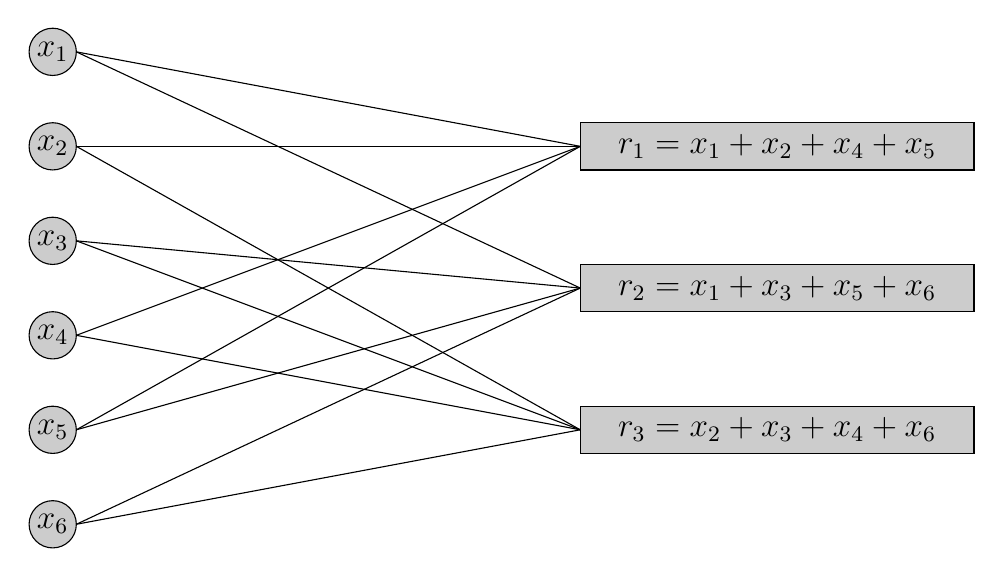
\begin{tikzpicture}
\fill [color=white,opacity=0] (0, 0) rectangle (12, -6.6);

\filldraw [fill=black!20!white] (0.3, -0.3) circle (0.3);
\node at (0.3, -0.3) [font=\fontsize{12pt}{20pt}\selectfont] {$x_1$};
\filldraw [fill=black!20!white] (0.3, -1.5) circle (0.3);
\node at (0.3, -1.5) [font=\fontsize{12pt}{20pt}\selectfont] {$x_2$};
\filldraw [fill=black!20!white] (0.3, -2.7) circle (0.3);
\node at (0.3, -2.7) [font=\fontsize{12pt}{20pt}\selectfont] {$x_3$};
\filldraw [fill=black!20!white] (0.3, -3.9) circle (0.3);
\node at (0.3, -3.9) [font=\fontsize{12pt}{20pt}\selectfont] {$x_4$};
\filldraw [fill=black!20!white] (0.3, -5.1) circle (0.3);
\node at (0.3, -5.1) [font=\fontsize{12pt}{20pt}\selectfont] {$x_5$};
\filldraw [fill=black!20!white] (0.3, -6.3) circle (0.3);
\node at (0.3, -6.3) [font=\fontsize{12pt}{20pt}\selectfont] {$x_6$};

\filldraw [fill=black!20!white] (7, -1.2) rectangle (12, -1.8);
\node at (9.5, -1.5) [font=\fontsize{12pt}{20pt}\selectfont] {$r_1=x_1+x_2+x_4+x_5$};
\filldraw [fill=black!20!white] (7, -3) rectangle (12, -3.6);
\node at (9.5, -3.3) [font=\fontsize{12pt}{20pt}\selectfont] {$r_2=x_1+x_3+x_5+x_6$};
\filldraw [fill=black!20!white] (7, -4.8) rectangle (12, -5.4);
\node at (9.5, -5.1) [font=\fontsize{12pt}{20pt}\selectfont] {$r_3=x_2+x_3+x_4+x_6$};

\draw (0.6, -0.3) -- (7, -1.5);
\draw (0.6, -1.5) -- (7, -1.5);
\draw (0.6, -3.9) -- (7, -1.5);
\draw (0.6, -5.1) -- (7, -1.5);
\draw (0.6, -0.3) -- (7, -3.3);
\draw (0.6, -2.7) -- (7, -3.3);
\draw (0.6, -5.1) -- (7, -3.3);
\draw (0.6, -6.3) -- (7, -3.3);
\draw (0.6, -1.5) -- (7, -5.1);
\draw (0.6, -2.7) -- (7, -5.1);
\draw (0.6, -3.9) -- (7, -5.1);
\draw (0.6, -6.3) -- (7, -5.1);
\end{tikzpicture}
}
\caption{LDPC 编码的 Tanner 图示意}
\label{p13}
\end{figure}
\subsection{里德-所罗门码}
里德-所罗门码(Reed-Solomon Codes)\cite{reed1960polynomial}是在存储系统中较为常用的一种纠删码算法,也是唯一一种可以使用任意数据块个数 $n$ 和任意冗余块个数 $m$ 进行编码的 MDS 编码方法。里德-所罗门码是一种基于有限域的编码算法,给定 $n$ 个数据块(Data block)$D_1$、$D_2$、$\cdots$、$D_n$,和一个正整数 $m$,里德-所罗门码根据 $n$ 个数据块生成 $m$ 个编码块(Code block)$C_1$、$C_2$、$\cdots$、$C_m$。在编码生成的全部 $n$ 个数据块和 $m$ 个编码块中,选取任意 $n$ 个块均能解码出原始数据,即里德-所罗门码最多容忍任意 $m$ 个数据块或者编码块同时丢失。上述里德-所罗门码中的变量 $D_i$、$C_i$ 代表字长 $w$ 为 8 位或者 16 位的字。较大的数据块需要先拆分为字,然后将字作为编码和解码的单位,对字进行编码和解码。

将原始数据记为向量 $\boldsymbol{D}=(D_1,D_2,\cdots,D_n)^{T}$,其经过里德-所罗门码编码生成的校验码为向量 $\boldsymbol{C}=(D_1,D_2,\cdots,D_n,C_1,C_2,\cdots,C_m)^{T}$,则里德-所罗门码的编码过程可视为矩阵运算 $\boldsymbol{G}{\times}\boldsymbol{D}=\boldsymbol{C}$,其中 $\boldsymbol{G}$ 是编码矩阵(Distribution Matrix,也可称为生成矩阵、分布矩阵)。由于解码是编码的逆运算,因此要求编码矩阵的任意 $n{\times}n$ 子方阵均为可逆矩阵。在里德-所罗门码的编码矩阵中,上部矩阵一般是 $n{\times}n$ 的单位阵,表示直接存储原始数据,下部矩阵是  $m{\times}n$ 的校验码矩阵。我们常选择范德蒙矩阵\cite{reed1960polynomial}或柯西矩阵\cite{roth1989mds}作为里德-所罗门码编码矩阵的下部矩阵。

范德蒙矩阵的各列间为等比级数关系,满足任意阶子方阵可逆的要求。一个 $m{\times}n$ 的范德蒙矩阵定义如下:
\begin{equation}
\begin{bmatrix}
1 & 1 & 1 & \cdots & 1 \\
{a_1}^1 & {a_2}^1 & {a_3}^1 & \cdots & {a_n}^1 \\
{a_1}^2 & {a_2}^2 & {a_3}^2 & \cdots & {a_n}^2 \\
\vdots & \vdots & \vdots & \ddots & \vdots \\
{a_1}^{m-1} & {a_2}^{m-1} & {a_3}^{m-1} & \cdots & {a_n}^{m-1} \\
\end{bmatrix}
\end{equation}
其中 $a_i$ 互不相同,且均不为 0。

柯西矩阵的任意阶子方阵均为奇异矩阵,因此其任意阶子方阵均存在逆矩阵。而且由于柯西矩阵在迦罗华域上求逆矩阵的计算复杂度为 $O(n^2)$,相比于范德蒙矩阵求逆的计算复杂度 $O(n^3)$ 更低,运算速度更快。另外,在使用柯西矩阵进行矩阵计算时,可以通过将 $GF(2^w)$ 域的元素转换成二进制矩阵,从而将乘法转换为位运算,进而降低编码运算的复杂度。柯西矩阵的定义为:
\begin{equation}
\begin{bmatrix}
\dfrac{1}{x_1+y_1} & \dfrac{1}{x_1+y_2} & \dfrac{1}{x_1+y_3} & \cdots & \dfrac{1}{x_1+y_n} \\
\dfrac{1}{x_2+y_1} & \dfrac{1}{x_2+y_2} & \dfrac{1}{x_2+y_3} & \cdots & \dfrac{1}{x_2+y_n} \\
\dfrac{1}{x_3+y_1} & \dfrac{1}{x_3+y_2} & \dfrac{1}{x_3+y_3} & \cdots & \dfrac{1}{x_3+y_n} \\
\vdots & \vdots & \vdots & \ddots & \vdots \\
\dfrac{1}{x_m+y_1} & \dfrac{1}{x_m+y_2} & \dfrac{1}{x_m+y_3} & \cdots & \dfrac{1}{x_m+y_n} \\
\end{bmatrix}
\end{equation}
其中 $x_i$ 和 $y_i$ 都是有限域 $GF(2^w)$ 中的元素。

里德-所罗门码在任意不超过 $m$ 个数据块丢失时均可进行数据恢复。如图 \ref{p1} 所示,假设其中的 $D_2$、$D_5$ 发生损坏,我们可以从编码矩阵 $\boldsymbol{G}$ 中删掉 $D_2$、$D_5$ 对应的行,组成新矩阵 $\boldsymbol{G_1}$。根据编码矩阵任意阶子方阵可逆可以证明 $\boldsymbol{G_1}$ 是可逆的,即存在逆矩阵 $(\boldsymbol{G_1})^{-1}$,满足 $\boldsymbol{G_1}{\times}(\boldsymbol{G_1})^{-1}=\boldsymbol{I}$,其中 $\boldsymbol{I}$ 为单位矩阵。将剩余未损坏的数据左乘 $(\boldsymbol{G_1})^{-1}$ 矩阵,便可以恢复出原始数据 $\boldsymbol{D}$。

\begin{figure}[!htb]
\centering
\resizebox{.8\textwidth}{!}{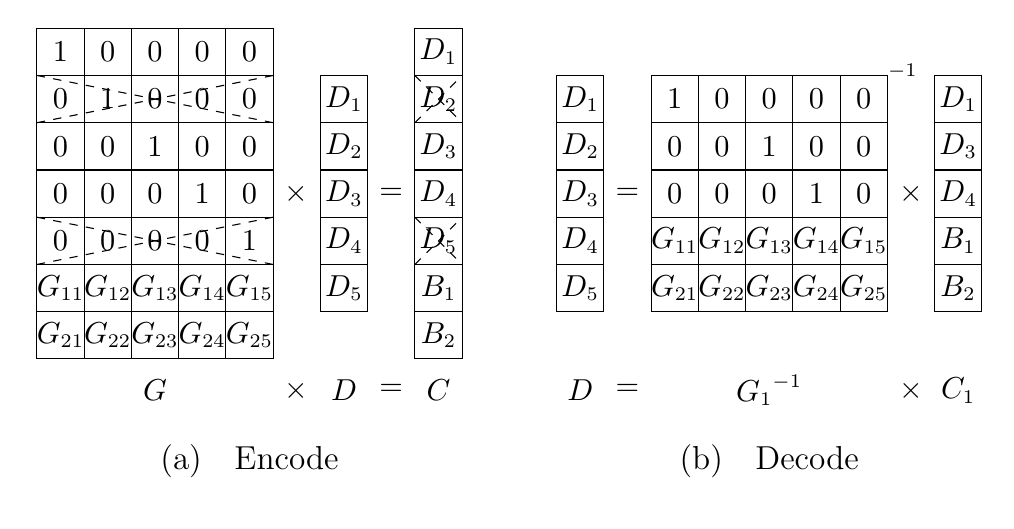
\begin{tikzpicture}
\fill [color=white,opacity=0] (0, 0) rectangle (12, 6);

\node at (2.7, 0.5) [font=\fontsize{12pt}{20pt}\selectfont] {(a){\quad}Encode};
\node at (1.5, 1.4) [font=\fontsize{10.5pt}{20pt}\selectfont] {$\boldsymbol{G}$};
\node at (3.3, 1.4) [font=\fontsize{10.5pt}{20pt}\selectfont] {$\times$};
\node at (3.9, 1.4) [font=\fontsize{10.5pt}{20pt}\selectfont] {$\boldsymbol{D}$};
\node at (4.5, 1.4) [font=\fontsize{10.5pt}{20pt}\selectfont] {$=$};
\node at (5.1, 1.4) [font=\fontsize{10.5pt}{20pt}\selectfont] {$\boldsymbol{C}$};

\draw (0, 1.8) rectangle (3, 6);
\foreach \x in {1,...,6} {
    \draw (0, 1.8+0.6*\x) -- (3, 1.8+0.6*\x);
}
\foreach \x in {1,...,4} {
    \draw (0.6*\x, 1.8) -- (0.6*\x, 6);
}
\node at (0.3, 5.7) [font=\fontsize{10.5pt}{20pt}\selectfont] {$1$};
\node at (0.9, 5.7) [font=\fontsize{10.5pt}{20pt}\selectfont] {$0$};
\node at (1.5, 5.7) [font=\fontsize{10.5pt}{20pt}\selectfont] {$0$};
\node at (2.1, 5.7) [font=\fontsize{10.5pt}{20pt}\selectfont] {$0$};
\node at (2.7, 5.7) [font=\fontsize{10.5pt}{20pt}\selectfont] {$0$};
\node at (0.3, 5.1) [font=\fontsize{10.5pt}{20pt}\selectfont] {$0$};
\node at (0.9, 5.1) [font=\fontsize{10.5pt}{20pt}\selectfont] {$1$};
\node at (1.5, 5.1) [font=\fontsize{10.5pt}{20pt}\selectfont] {$0$};
\node at (2.1, 5.1) [font=\fontsize{10.5pt}{20pt}\selectfont] {$0$};
\node at (2.7, 5.1) [font=\fontsize{10.5pt}{20pt}\selectfont] {$0$};
\node at (0.3, 4.5) [font=\fontsize{10.5pt}{20pt}\selectfont] {$0$};
\node at (0.9, 4.5) [font=\fontsize{10.5pt}{20pt}\selectfont] {$0$};
\node at (1.5, 4.5) [font=\fontsize{10.5pt}{20pt}\selectfont] {$1$};
\node at (2.1, 4.5) [font=\fontsize{10.5pt}{20pt}\selectfont] {$0$};
\node at (2.7, 4.5) [font=\fontsize{10.5pt}{20pt}\selectfont] {$0$};
\node at (0.3, 3.9) [font=\fontsize{10.5pt}{20pt}\selectfont] {$0$};
\node at (0.9, 3.9) [font=\fontsize{10.5pt}{20pt}\selectfont] {$0$};
\node at (1.5, 3.9) [font=\fontsize{10.5pt}{20pt}\selectfont] {$0$};
\node at (2.1, 3.9) [font=\fontsize{10.5pt}{20pt}\selectfont] {$1$};
\node at (2.7, 3.9) [font=\fontsize{10.5pt}{20pt}\selectfont] {$0$};
\node at (0.3, 3.3) [font=\fontsize{10.5pt}{20pt}\selectfont] {$0$};
\node at (0.9, 3.3) [font=\fontsize{10.5pt}{20pt}\selectfont] {$0$};
\node at (1.5, 3.3) [font=\fontsize{10.5pt}{20pt}\selectfont] {$0$};
\node at (2.1, 3.3) [font=\fontsize{10.5pt}{20pt}\selectfont] {$0$};
\node at (2.7, 3.3) [font=\fontsize{10.5pt}{20pt}\selectfont] {$1$};
\node at (0.3, 2.7) [font=\fontsize{10.5pt}{20pt}\selectfont] {$G_{11}$};
\node at (0.9, 2.7) [font=\fontsize{10.5pt}{20pt}\selectfont] {$G_{12}$};
\node at (1.5, 2.7) [font=\fontsize{10.5pt}{20pt}\selectfont] {$G_{13}$};
\node at (2.1, 2.7) [font=\fontsize{10.5pt}{20pt}\selectfont] {$G_{14}$};
\node at (2.7, 2.7) [font=\fontsize{10.5pt}{20pt}\selectfont] {$G_{15}$};
\node at (0.3, 2.1) [font=\fontsize{10.5pt}{20pt}\selectfont] {$G_{21}$};
\node at (0.9, 2.1) [font=\fontsize{10.5pt}{20pt}\selectfont] {$G_{22}$};
\node at (1.5, 2.1) [font=\fontsize{10.5pt}{20pt}\selectfont] {$G_{23}$};
\node at (2.1, 2.1) [font=\fontsize{10.5pt}{20pt}\selectfont] {$G_{24}$};
\node at (2.7, 2.1) [font=\fontsize{10.5pt}{20pt}\selectfont] {$G_{25}$};

\node at (3.3, 3.9) [font=\fontsize{10.5pt}{20pt}\selectfont] {$\times$};

\draw (3.6, 2.4) rectangle (4.2, 5.4);
\foreach \x in {1,...,4} {
    \draw (3.6, 2.4+0.6*\x) -- (4.2, 2.4+0.6*\x);
}
\node at (3.9, 5.1) [font=\fontsize{10.5pt}{20pt}\selectfont] {$D_{1}$};
\node at (3.9, 4.5) [font=\fontsize{10.5pt}{20pt}\selectfont] {$D_{2}$};
\node at (3.9, 3.9) [font=\fontsize{10.5pt}{20pt}\selectfont] {$D_{3}$};
\node at (3.9, 3.3) [font=\fontsize{10.5pt}{20pt}\selectfont] {$D_{4}$};
\node at (3.9, 2.7) [font=\fontsize{10.5pt}{20pt}\selectfont] {$D_{5}$};

\node at (4.5, 3.9) [font=\fontsize{10.5pt}{20pt}\selectfont] {$=$};

\draw (4.8, 1.8) rectangle (5.4, 6);
\foreach \x in {1,...,6} {
    \draw (4.8, 1.8+0.6*\x) -- (5.4, 1.8+0.6*\x);
}
\node at (5.1, 5.7) [font=\fontsize{10.5pt}{20pt}\selectfont] {$D_{1}$};
\node at (5.1, 5.1) [font=\fontsize{10.5pt}{20pt}\selectfont] {$D_{2}$};
\node at (5.1, 4.5) [font=\fontsize{10.5pt}{20pt}\selectfont] {$D_{3}$};
\node at (5.1, 3.9) [font=\fontsize{10.5pt}{20pt}\selectfont] {$D_{4}$};
\node at (5.1, 3.3) [font=\fontsize{10.5pt}{20pt}\selectfont] {$D_{5}$};
\node at (5.1, 2.7) [font=\fontsize{10.5pt}{20pt}\selectfont] {$B_{1}$};
\node at (5.1, 2.1) [font=\fontsize{10.5pt}{20pt}\selectfont] {$B_{2}$};

\draw [dashed] (0, 3) -- (3, 3.6);
\draw [dashed] (0, 3.6) -- (3, 3);
\draw [dashed] (0, 4.8) -- (3, 5.4);
\draw [dashed] (0, 5.4) -- (3, 4.8);
\draw [dashed] (4.8, 3) -- (5.4, 3.6);
\draw [dashed] (4.8, 3.6) -- (5.4, 3);
\draw [dashed] (4.8, 4.8) -- (5.4, 5.4);
\draw [dashed] (4.8, 5.4) -- (5.4, 4.8);

\node at (9.3, 0.5) [font=\fontsize{12pt}{20pt}\selectfont] {(b){\quad}Decode};
\node at (6.9, 1.4) [font=\fontsize{10.5pt}{20pt}\selectfont] {$\boldsymbol{D}$};
\node at (7.5, 1.4) [font=\fontsize{10.5pt}{20pt}\selectfont] {$=$};
\node at (9.3, 1.4) [font=\fontsize{10.5pt}{20pt}\selectfont] {$\boldsymbol{G_{1}}^{-1}$};
\node at (11.1, 1.4) [font=\fontsize{10.5pt}{20pt}\selectfont] {$\times$};
\node at (11.7, 1.4) [font=\fontsize{10.5pt}{20pt}\selectfont] {$\boldsymbol{C_{1}}$};

\draw (6.6, 2.4) rectangle (7.2, 5.4);
\foreach \x in {1,...,4} {
    \draw (6.6, 2.4+0.6*\x) -- (7.2, 2.4+0.6*\x);
}
\node at (6.9, 5.1) [font=\fontsize{10.5pt}{20pt}\selectfont] {$D_{1}$};
\node at (6.9, 4.5) [font=\fontsize{10.5pt}{20pt}\selectfont] {$D_{2}$};
\node at (6.9, 3.9) [font=\fontsize{10.5pt}{20pt}\selectfont] {$D_{3}$};
\node at (6.9, 3.3) [font=\fontsize{10.5pt}{20pt}\selectfont] {$D_{4}$};
\node at (6.9, 2.7) [font=\fontsize{10.5pt}{20pt}\selectfont] {$D_{5}$};

\node at (7.5, 3.9) [font=\fontsize{10.5pt}{20pt}\selectfont] {$=$};

\draw (7.8, 2.4) rectangle (10.8, 5.4);
\foreach \x in {1,...,4} {
    \draw (7.8, 2.4+0.6*\x) -- (10.8, 2.4+0.6*\x);
}
\foreach \x in {1,...,4} {
    \draw (7.8+0.6*\x, 2.4) -- (7.8+0.6*\x, 5.4);
}
\node at (8.1, 5.1) [font=\fontsize{10.5pt}{20pt}\selectfont] {$1$};
\node at (8.7, 5.1) [font=\fontsize{10.5pt}{20pt}\selectfont] {$0$};
\node at (9.3, 5.1) [font=\fontsize{10.5pt}{20pt}\selectfont] {$0$};
\node at (9.9, 5.1) [font=\fontsize{10.5pt}{20pt}\selectfont] {$0$};
\node at (10.5, 5.1) [font=\fontsize{10.5pt}{20pt}\selectfont] {$0$};
\node at (8.1, 4.5) [font=\fontsize{10.5pt}{20pt}\selectfont] {$0$};
\node at (8.7, 4.5) [font=\fontsize{10.5pt}{20pt}\selectfont] {$0$};
\node at (9.3, 4.5) [font=\fontsize{10.5pt}{20pt}\selectfont] {$1$};
\node at (9.9, 4.5) [font=\fontsize{10.5pt}{20pt}\selectfont] {$0$};
\node at (10.5, 4.5) [font=\fontsize{10.5pt}{20pt}\selectfont] {$0$};
\node at (8.1, 3.9) [font=\fontsize{10.5pt}{20pt}\selectfont] {$0$};
\node at (8.7, 3.9) [font=\fontsize{10.5pt}{20pt}\selectfont] {$0$};
\node at (9.3, 3.9) [font=\fontsize{10.5pt}{20pt}\selectfont] {$0$};
\node at (9.9, 3.9) [font=\fontsize{10.5pt}{20pt}\selectfont] {$1$};
\node at (10.5, 3.9) [font=\fontsize{10.5pt}{20pt}\selectfont] {$0$};
\node at (8.1, 3.3) [font=\fontsize{10.5pt}{20pt}\selectfont] {$G_{11}$};
\node at (8.7, 3.3) [font=\fontsize{10.5pt}{20pt}\selectfont] {$G_{12}$};
\node at (9.3, 3.3) [font=\fontsize{10.5pt}{20pt}\selectfont] {$G_{13}$};
\node at (9.9, 3.3) [font=\fontsize{10.5pt}{20pt}\selectfont] {$G_{14}$};
\node at (10.5, 3.3) [font=\fontsize{10.5pt}{20pt}\selectfont] {$G_{15}$};
\node at (8.1, 2.7) [font=\fontsize{10.5pt}{20pt}\selectfont] {$G_{21}$};
\node at (8.7, 2.7) [font=\fontsize{10.5pt}{20pt}\selectfont] {$G_{22}$};
\node at (9.3, 2.7) [font=\fontsize{10.5pt}{20pt}\selectfont] {$G_{23}$};
\node at (9.9, 2.7) [font=\fontsize{10.5pt}{20pt}\selectfont] {$G_{24}$};
\node at (10.5, 2.7) [font=\fontsize{10.5pt}{20pt}\selectfont] {$G_{25}$};

\node at (11, 5.4) [font=\fontsize{10.5pt}{20pt}\selectfont] {$^{-1}$};

\node at (11.1, 3.9) [font=\fontsize{10.5pt}{20pt}\selectfont] {$\times$};

\draw (11.4, 2.4) rectangle (12, 5.4);
\foreach \x in {1,...,4} {
    \draw (11.4, 2.4+0.6*\x) -- (12, 2.4+0.6*\x);
}
\node at (11.7, 5.1) [font=\fontsize{10.5pt}{20pt}\selectfont] {$D_{1}$};
\node at (11.7, 4.5) [font=\fontsize{10.5pt}{20pt}\selectfont] {$D_{3}$};
\node at (11.7, 3.9) [font=\fontsize{10.5pt}{20pt}\selectfont] {$D_{4}$};
\node at (11.7, 3.3) [font=\fontsize{10.5pt}{20pt}\selectfont] {$B_{1}$};
\node at (11.7, 2.7) [font=\fontsize{10.5pt}{20pt}\selectfont] {$B_{2}$};
\end{tikzpicture}
}
\caption{纠删码编码和解码示意}
\label{p1}
\end{figure}
\section{基于纠删码的分布式存储系统}
\subsection{常见分布式存储系统的纠删码实现}
由于在分布式存储系统中应用多副本备份时数据冗余度较高,因此为了降低数据的冗余度,在保证数据安全的前提下降低存储成本,因此可以采用纠删码进行数据的存储。由于在常见的纠删码编码方案中,只有里德-所罗门码是可以基于任意数据块个数和校验块个数进行编码的纠删码方案,相比其他纠删码方案更加灵活,因此,在分布式存储系统中,一般采用里德-所罗门码进行数据的纠删码编码。
\subsubsection{里德-所罗门码在常见分布式存储系统中的应用}
目前主流分布式存储系统均使用里德-所罗门码纠删码编码方案进行冗余备份。以 $n=4$,$m=2$ 的里德-所罗门码纠删码方案为例,其可以容忍最多两个数据块的丢失,因此具有与三副本备份方案相近的容错能力,但纠删码方案的数据冗余度仅为 $50\%$,大大低于多副本备份的数据冗余度。但当使用纠删码编码的存储系统发生数据损坏时,存储系统需要通过至少 $n$ 个块计算重建数据,相比多副本备份的直接拷贝需要额外的计算资源开销,也占用了更多的磁盘带宽和网络带宽。根据 Arafa 等人\cite{arafa2018evaluating}的研究,在主流的分布式文件系统 HDFS 和 Ceph 中,使用纠删码引擎进行存储均有明显的性能损失。因此若要在存储系统中广泛应用纠删码技术,需要研究更加高效的方案,比如提高系统并行度等,以解决纠删码的性能瓶颈问题。
\subsubsection{Ceph 分布式文件系统的纠删码存储方案}
在 Ceph 分布式文件系统中,其纠删码引擎应用 Jerasure 函数库实现,当管理员创建基于纠删码的存储后端时,可以指定数据块数量 $n$ 和编码块数量 $m$ 作为系统的参数。在纠删码存储后端中,每个数据对象都被分成 $n$ 个数据块和 $m$ 个编码块,分别存放于 $n+m$ 个对象存储设备(Object Storage Device,即 OSD)中。因此在 Ceph 分布式文件系统中,对于所有对象均采用相同的数据块和编码块数量,没有动态地考虑对象的需求和存储设备的条件。
\subsubsection{Ceph 分布式文件系统的纠删码数据的修改}
在基于纠删码的数据修改方面,由于纠删码的编解码开销过大,导致 Ceph 难以简单地实现数据修改。Ceph 采用元数据服务器(Metadata Server,即 MDS)主要负责 CephFS 集群中文件和目录的管理,记录数据的属性,如文件存储位置、大小、存储时间等,同时负责文件查找、文件记录、存储位置记录、访问授权等。Ceph 的 Bluestore\cite{aghayev2019file} OSD 在最新的 Luminous 版本增加了部分写入功能,可以将 Ceph 的文件数据存储在纠删码存储池中。然而由于覆盖写入需要对对象做出修改,增加了系统的复杂性,且由于需要进行解码和重新编码,写入效率不高。
\subsubsection{Hadoop 分布式文件系统的纠删码数据的修改}
在 HDFS 的早期版本中,为了与 MapReduce 配合,同样不支持文件附加或者文件修改。但在最新的 Hadoop 2.x 版本中,HDFS 新增支持了文件附加操作。
\subsubsection{GFS 分布式文件系统的纠删码数据的修改}
在 GFS 中,每个大文件被划分为若干个固定大小的块,其写操作主要分为写入和附加两种。其中写入操作是修改数据,附加操作则是在文件末尾添加数据。但 GFS 的前提假设是文件系统的写操作主要是对文件进行追加操作, 追加的数据是足够大且顺序追加的,在写入后文件就很少会被修改。虽然 GFS 支持小的随机写入,但并不是文件系统优化的目标。同时 GFS 的写入必须是原子操作,一次写入的数据必须是原子性的添加到文件结尾。若有两个独立的进程 A 和 B 同时附加数据到同一个文件里,由于需要寻找文件末尾的位置后才能添加数据,会产生互斥问题。
\subsection{分布式文件系统中纠删码运算效率的研究}
由于基于里德-所罗门码的纠删码编码和解码需要较高的额外资源开销,因此需要我们对编码运算和编码策略进行优化,从而实现高效的分布式文件系统。

在编码运算优化方面,最基础的便是对矩阵运算进行优化。由于柯西矩阵的求逆矩阵的计算复杂度更低,且在有限域 $GF(2^w)$ 上进行的运算更加容易优化,因此可以利用柯西矩阵代替范德蒙矩阵提高编码和解码效率。针对不同数据的纠删码编码可以并行计算的特点,Liu 等\cite{liu2018g}提出了 G-CRS,其采用柯西矩阵进行纠删码的编码,并通过 GPU 加速基于柯西矩阵的里德-所罗门码纠删码的计算。通过在基于 Maxwell 和 Pascal 等架构的现代 GPU 上的实验结果显示,G-CRS 的数据吞吐量比目前大多数基于 CPU 的编码库快 10 倍。针对在纠删码解码过程中需要先通过解码矩阵计算原始数据,才能根据编码矩阵进行校验块的计算的问题,Fan 等\cite{fan2019new}提出了一种新的计算方案,其可以同时计算原始数据块和冗余编码块。Zhou 等\cite{zhou2019fast}还提出了一种结合改进编码矩阵、减少计算中相同的 XOR 操作、优化计算调度算法、高效管理 cache 和矢量化等技术的方法,来提高纠删码的编码效率。

此外,针对不同数据块和不同存储设备之间存在差异的特点,我们可以通过动态的纠删码编码策略来代替固定的纠删码编码策略,从而对系统进行优化。Abebe 等\cite{abebe2018ec}提出了一种在纠删码分布式存储系统中,基于工作负载访问模式进行数据访问和数据移动的策略 EC-Store,并通过在两个基准测试上的评估,证明其可以显著地减少数据检索的开销。针对大规模集群存储系统通常为异构存储架构,常常是使用可靠性存在差异的不同存储设备混合组成的特点,Kadekodi 等\cite{kadekodi2019cluster}提出了 HeART,通过读取磁盘的属性信息,来估计磁盘的长期数据可靠性,并基于此尽可能地减少备份数据的存储。Xiang 等\cite{xiang2015joint}提出了一种通过联合考虑存储系统延迟和开销来优化纠删码编码的方案。Plank 等\cite{plank2014sector}提出了 SD Codes 来区别对待整个磁盘故障和磁盘部分扇区故障,提高存储效率。Zhang 等\cite{zhang2019nade}提出了 NADE 模型对节点数据读取进行优化。
\subsection{分布式文件系统中的纠删码数据修改的研究}
由于基于里德-所罗门码的纠删码的分布式文件系统在数据进行修改时需要重新编解码,因此一般均用于存储只读的对象数据。但是,在实际的数据存储需求中,对于数据的修改是很常见的。因此,如何在基于里德-所罗门码的纠删码分布式文件系统上实现一个快速的可读写的存储系统,是分布式文件系统领域研究的热点问题之一。

针对在对象存储上支持块存储,Gutierrez 等\cite{gutierrez2017ustorage}提出了 uStorage 方案,作者认为块级存储广泛用于支持繁重的工作负载。它可以由操作系统直接访问,但它在分布式系统中面临一些持久性问题、硬件限制和性能下降。基于对象的存储设备(OSD)是一种广泛用于支持一次写入多次读取(WORM)系统的数据存储概念。由于 OSD 包含数据、元数据和唯一标识符,因此它变得非常强大且可自定义。 OSD 是解决日益增长的数据增长和弹性需求问题,同时降低成本的理想选择。作者描述了一种可扩展的存储架构,该架构使用来自分布式 P2P 云存储系统的 OSD,并为用户提供块级存储层。该架构将商用硬件上 OSD 的备份、可靠性和可扩展性的优势与数据密集型工作负载的原始块的简单性相结合,展示了在后端使用 OSD 并基于原始块提供存储层的可能性,并为最终用户提供更好的性能,并基于缓存行为评估了所提出的架构,使用不同的高速缓存大小测量了两个存储层的繁重工作负载的高吞吐量性能。

在分布式文件系统的元数据存储方面,LocoFS 提出了一个分布式文件系统来提供松散耦合的元数据服务\cite{li2017locofs},以弥合文件系统元数据和键值存储之间的性能差距。LocoFS 旨在通过两种技术来分离不同类型的元数据之间的依赖关系。首先,LocoFS 解耦目录内容和结构,它在平面空间中组织文件和目录索引节点,同时反向索引目录条目。其次,它将文件元数据分离,以进一步提高键值访问性能。评估显示,具有八个节点的 LocoFS 将元数据吞吐量提高了 5 倍,单个节点键值存储的吞吐量接近 $93\%$,而最先进的 IndexFS 则为 $18\%$。

随着互联网的发展,分布式文件系统中开始存储了大量的图片,且这些图片的大小通常不超过 1 MB。为了满足包含这么多图片的小文件存储系统的需求,Chen 等\cite{chen2017erasure}提出了将小文件合并为块进行索引,并存储于纠删码后端的方案。实验表明,当系统容量为 1 PB 时,名称服务器中块信息的内存使用量小于 2 GB,显示了良好的可扩展性。同时,相比于两副本备份,使用纠删码降低了 $25\%$ 的存储开销,大大降低了存储成本。
\section{小结}
本章从数据常见的损坏方式出发,首先介绍了对应的几种数据恢复方法,如硬件恢复、多副本备份和纠删码备份等。针对于分布式存储系统中多副本备份冗余度高,存储资源浪费严重的特点,详细地介绍了常见的几种纠删码的定义和实现方式,并介绍了基于纠删码备份的分布式存储系统的优化方法。最后,针对分布式存储系统中纠删码实现在数据存储和恢复时需要解码并重新编码的特点,介绍了在基于纠删码实现的分布式存储系统中实现文件修改的方法以及文件存储结构相关的研究。
